\documentclass[10pt]{article}

% Lines beginning with the percent sign are comments
% This file has been commented to help you understand more about LaTeX

% DO NOT EDIT THE LINES BETWEEN THE TWO LONG HORIZONTAL LINES

%---------------------------------------------------------------------------------------------------------

% Packages add extra functionality.
\usepackage{
	times,
	graphicx,
	epstopdf,
	fancyhdr,
	amsfonts,
	amsthm,
	amsmath,
	algorithm,
	algorithmic,
	xspace,
	hyperref,
        qtree}
\usepackage[left=1in,top=1in,right=1in,bottom=1in]{geometry}
\usepackage{sect sty}	%For centering section headings
\usepackage{enumerate}	%Allows more labeling options for enumerate environments 
\usepackage{epsfig}
\usepackage[space]{grffile}
\usepackage{booktabs}
\usepackage{amsmath}
\usepackage[super]{nth}

% This will set LaTeX to look for figures in the same directory as the .tex file
\graphicspath{.} % The dot means current directory.

\pagestyle{fancy}

\lhead{\YOURID}
\chead{\projectName: Language Specification}
\rhead{\today}
\lfoot{CSCI 334: Principles of Programming Languages}
\cfoot{\thepage}
\rfoot{Spring 2020}

% Some commands for changing header and footer format
\renewcommand{\headrulewidth}{0.4pt}
\renewcommand{\headwidth}{\textwidth}
\renewcommand{\footrulewidth}{0.4pt}

% These let you use common environments
\newtheorem{claim}{Claim}
\newtheorem{definition}{Definition}
\newtheorem{theorem}{Theorem}
\newtheorem{lemma}{Lemma}
\newtheorem{observation}{Observation}
\newtheorem{question}{Question}

\setlength{\parindent}{0cm}
%---------------------------------------------------------------------------------------------------------

% DON'T CHANGE ANYTHING ABOVE HERE

% Edit below as instructed
\newcommand{\YOURID}{Petros Markopoulos}	% Replace "Your Name Here" with your name
\newcommand{\projectName}{\textbf{FUNny }}
\newcommand{\langName}{\textbf{FUNny Language }}
\newcommand{\intName}{\textbf{FUNny Visual Interface }}
\newcommand{\ProblemHeader}	% Don't change this!

\begin{document}

\vspace{\baselineskip}	% Add some vertical space

% Refer to the lab handouts to determine what should go in each of these sections.  Each lab is additive.  So lab 8 should include everything you wrote in lab 7.  Lab 9 should include everything you wrote in lab 8, etc.

\section{Introduction}
In this course we have spent a decent chunk of our time looking at the advantages of functional programming. We first discussed LISP and the innovations it brought, then we looked at the reading "Why Functional Programming Matters", which gave a detailed account of some benefits of functional programming and now we are learning F\#. It is safe to say, then, that functional programming is the unofficial theme of this course. But, if functional programming is so useful, why was it unfamiliar to most of us before this class? Why is it regarded as something complex and scary when it is neither, when, in fact, at its core it is very simple and elegant? In my view it is because it is because it is not introduced early in a programmer's life and so, when the time comes for one to learn it, they are already familiar with other common programming paradigms and they have a hard time adapting to the new way of thinking and coding.\\\\
This is the problem that my project, named \projectName, is aiming to solve. \projectName\ will consist of a simple functional programming language, and a visual programming environment for that language. The visual environment will work based on the simple view of functions as machines that transform the input given to them into output, just like we have seen multiple times in class. The programmer will have some pre-built machines at their disposal and the ability to compose them by piping their outputs to other machines in order to create more complex machines. \projectName\ is aimed mainly to children as an introduction to functional programming. It's goal is to demystify functional programming, illustrate the simplicity of its core concepts in a fun, enjoyable way and facilitate its learning, just like visual programming environments like Scratch are helpful as introductions to the imperative paradigm.


\section{Design Principles}
Naturally, \langName will be a simple functional programming language. It will be based on the idea of pure functions and declarative statements. My aim is for the code to be highly readable and descriptive, so as to facilitate the understanding of the code and its correlation with the \intName by younger children who may have a hard time reading sybmolic expressions. Since the \langName is not meant to be written, but rather generated using the \intName, it can be very strict in its form (the use of whitespace for example), since automatically generating consistent code is fairly simple.\\\\
\intName will be a visual interface utilizing the analogy between functions and machines that convert input into output. What will guide the implementation of the \intName will be the design of the \langName, as I would like them to feel strongly correlated, and also its design highly depends on the features that end up being implemented in the language. Aesthetically speaking, the \intName will be minimalistic, not only because I find that style to be pleasing, but also because I lack the ability to create any more intricate design.


\clearpage
\section{Example Programs}
\begin{enumerate}
    \item
        \[
            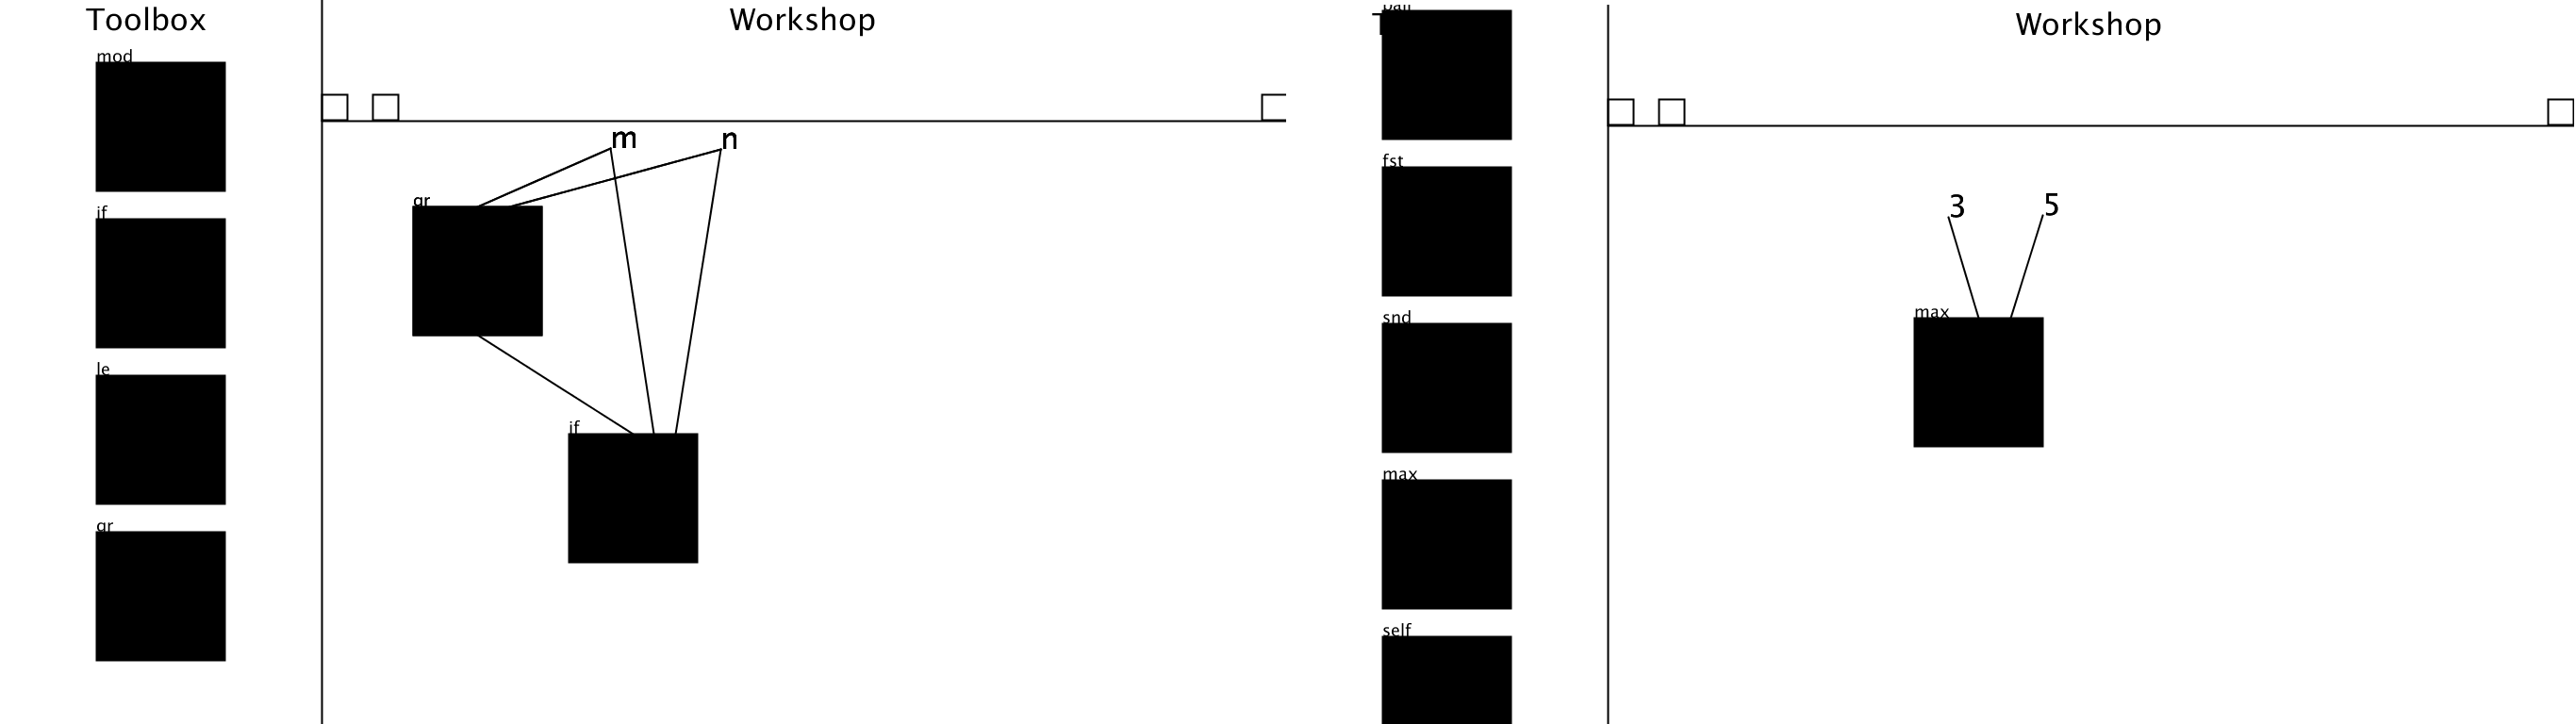
\includegraphics[width=\textwidth]{funny_program_example_1_visual_complete.png}
        \]
            In the left picture above, a new function is defined, which finds the maximum of two numbers. And in the right one, it is called with the arguments 3 and 5.\\
        The text of the program that the above generates is
        \[
            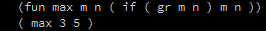
\includegraphics[width=\textwidth]{funny_program_example_1_text.png}
        \]
        The above program is created and run as follows:\\
        First, we start the \intName. Then we drag and drop the appropriate functions into the Workshop section and create the variables $m$ and $n$ by clicking on the button on the top right of the screen. We connect the variables and functions appropriately by first clicking on what we want to be the input and then on the object that is supposed to receive the input. After everything is connected, we click the leftmost button and type in the name "max" for our function and hit RETURN to save it in our toolbox. We drag and drop it in the Workshop area, create the values 3 and 5 and connect them to the function. After that, we hit the second button on the top left to run the program, and it should display the value 5.\\
        Alternatively it can be run with the command "dotnet run program" where program is the text representation shown above, all put in one line, with an extra "\\n" preceding each line of code.
    \item
        \[
            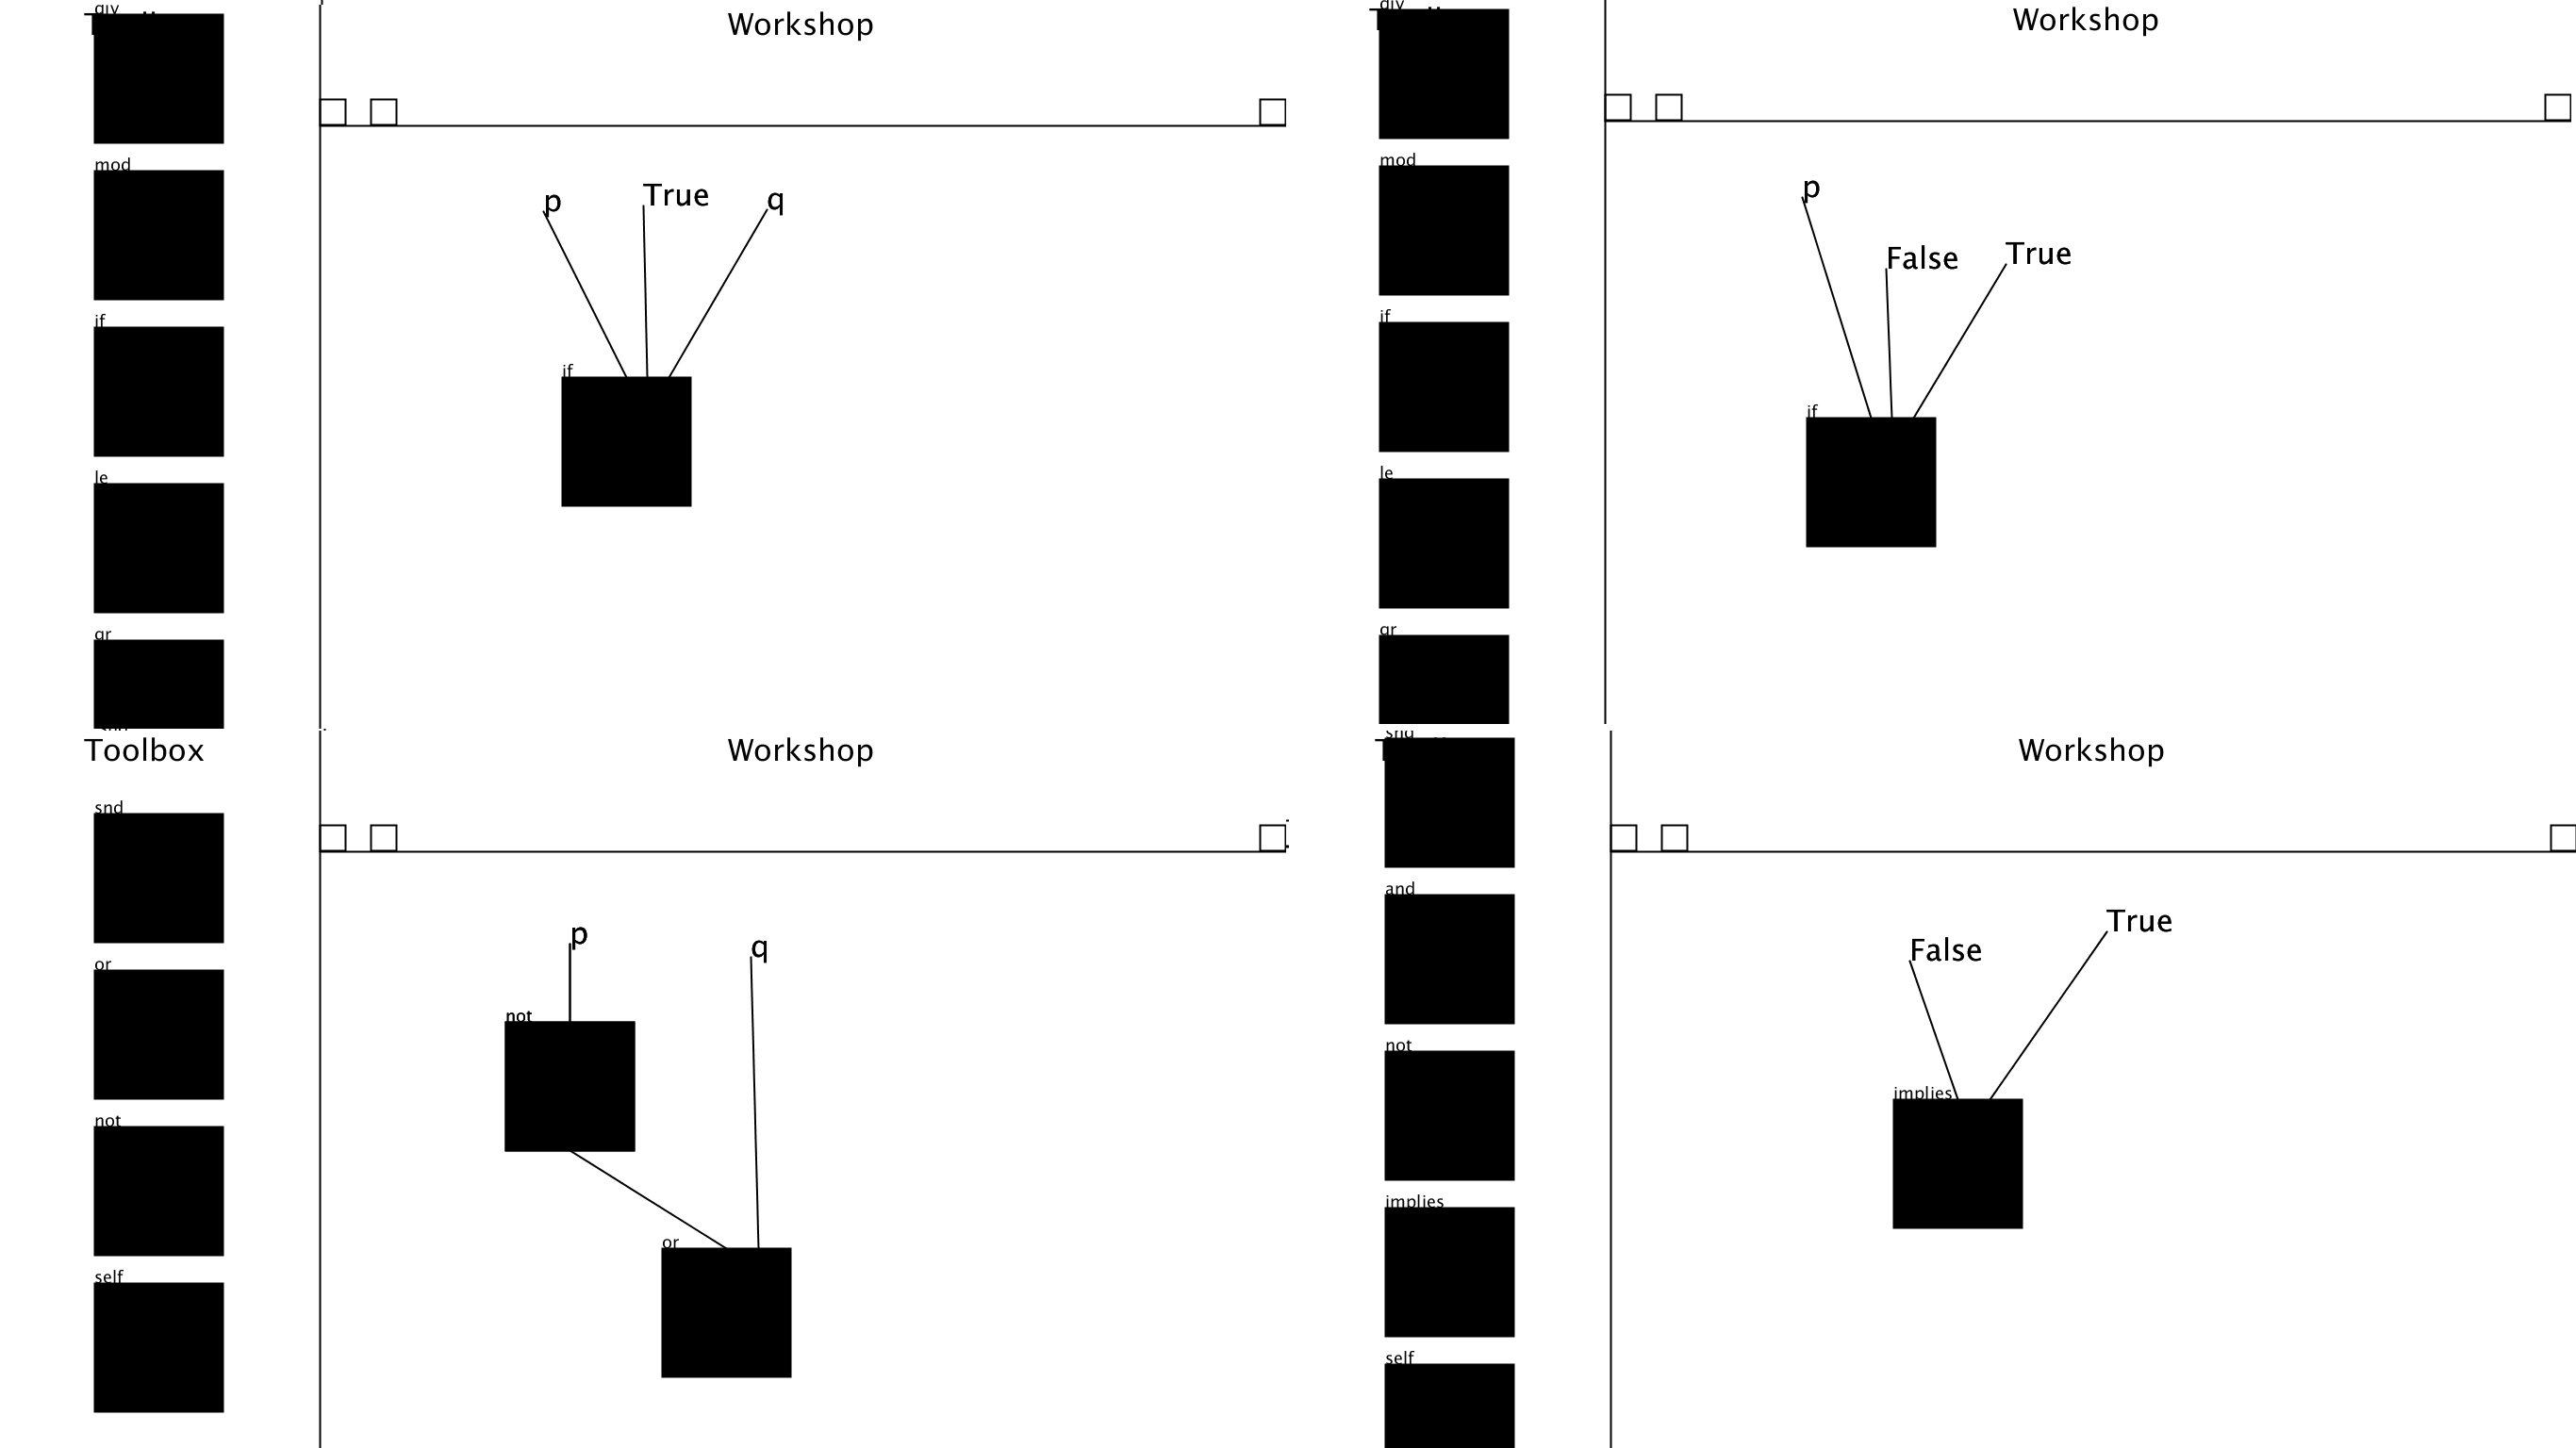
\includegraphics[width=\textwidth]{funny_program_example_2_visual_complete.png}
        \]
            In the top two picture above, some new functions is defined: the boolean operators \emph{or, not}. In the lower-left one, they are combined to define the function \emph{implies} which calculates the matching logic operator for two values. Then \emph{implies} is called with the arguments False and True.\\
        The text of the program that the above generates is
        \[
            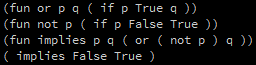
\includegraphics[width=\textwidth]{funny_program_example_2_text.png}
        \]
        To create the above program we do as follows:\\
        In any order we want, we build the three helper functions ("or", "not", "implies") in a manner similar to how we created "max" in the previous example. Then we drag and drop "implies" into the Workshop area, create the values False and True and connect them to the function. We click the run button and the outpu "True" should be displayed.\\
        Alternatively it can be run with the command "dotnet run program" where program is the text representation shown above, all put in one line, with an extra "\\n" preceding each line of code.
    \item
        \[
            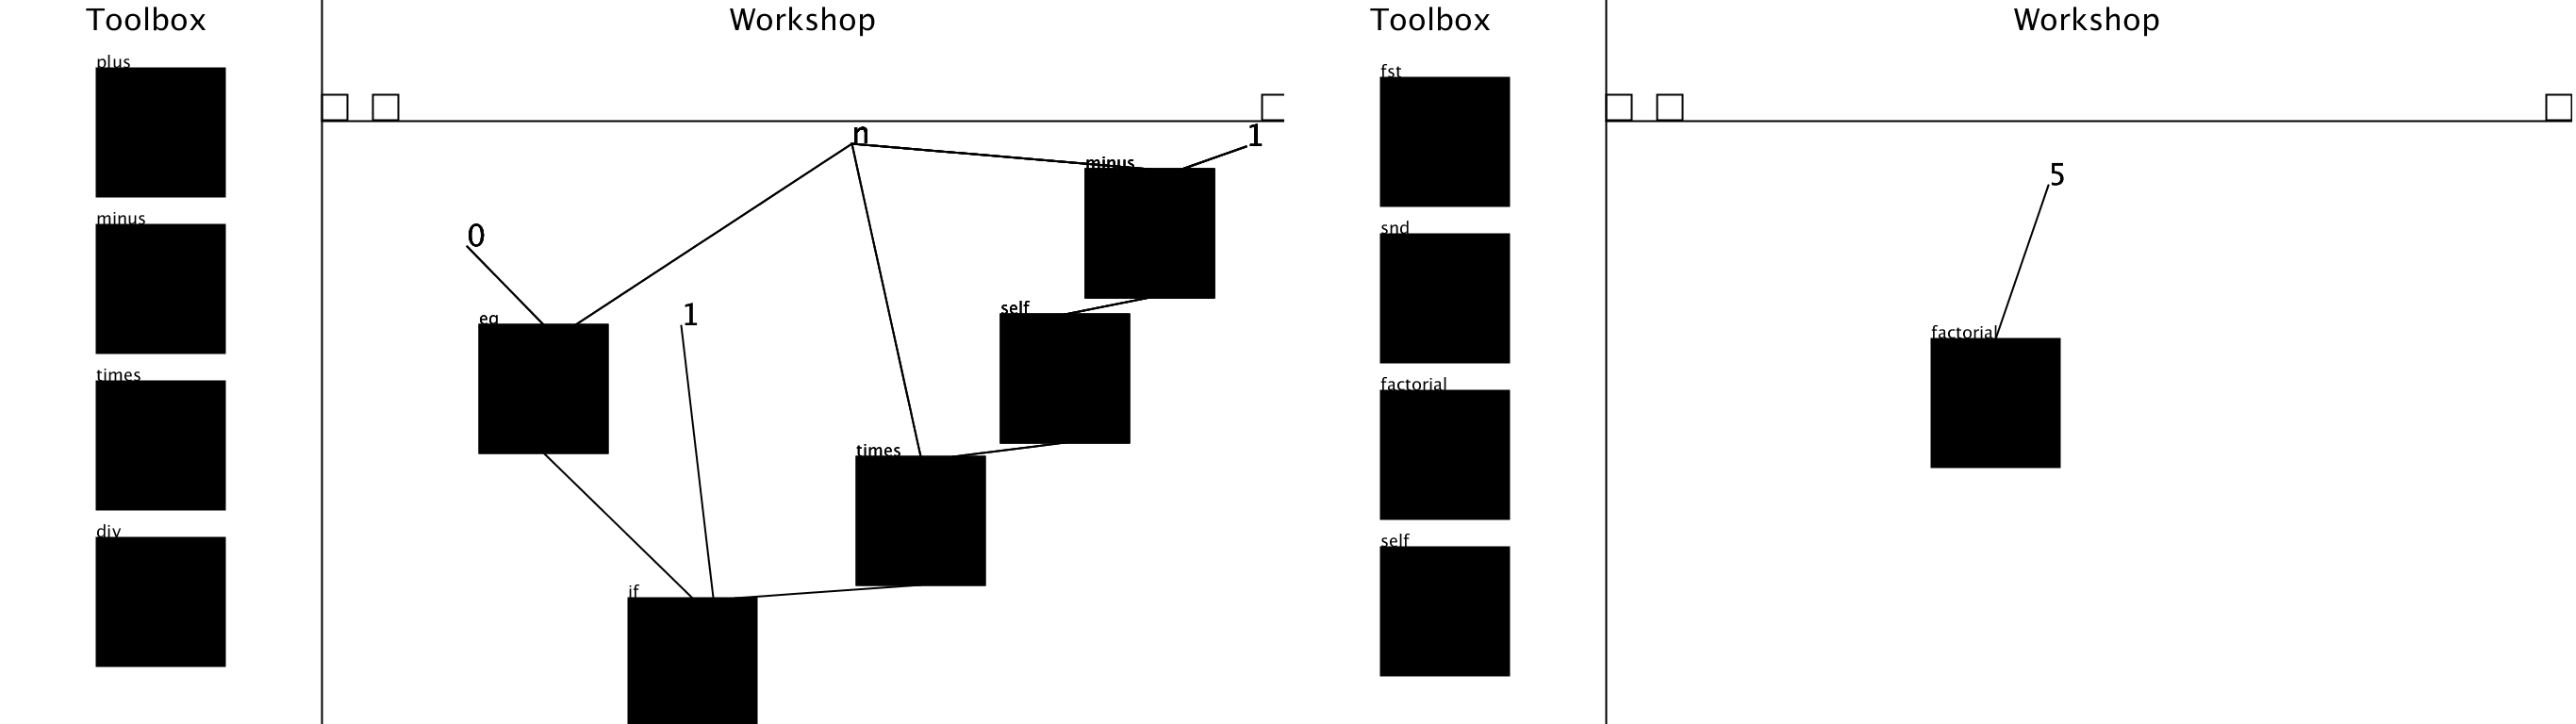
\includegraphics[width=\textwidth]{funny_program_example_3_visual_complete.png}
        \]
            In the left picture above, a new function is defined, which finds the factorial of a number. And in the right one, it is called with the argument 5.\\
        The text of the program that the above generates is
        \[
            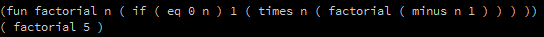
\includegraphics[width=\textwidth]{funny_program_example_3_text.png}
        \]
        The above program is built and run exactly like the two previous examples and should display the output 120 when run. It also illustrates the ease with which recursive functions are created in the \langName. The function "self" is dragged and dropped in the Workspace area and it stands in for the function that is being built as a whole. Any recursive call is, therefore, represented by passing the arguments that should be passed to the function to "self" instead and, similarly, using the output of "self" as one would use the output of the recursive call.\\
        Alternatively it can be run with the command "dotnet run program" where program is the text representation shown above, all put in one line, with an extra "\\n" preceding each line of code.
\end{enumerate}


\section{Language Concepts}
The most essential concept that needs to be understood is input and output. All that the \intName does is allow the user to connect inputs to functions and use the function's output as a new value to develop more complex functionality. An input can be any of the primitive values of the \langName (Int, Real, Boolean, Pair and Nil) which, with the exception of Nil are pretty intuitive. Nil represents the empty list in the \langName but it can also be thought of as the terminating element of a list. It is a very important concept to be understood as it is the key to creating lots of recursive functions on lists.\\
The combining form of the \langName is functions. Currently the \langName supports of functions of all primitive values. They are always pure functions, meaning that their only effect when given an input is to produce an output. There is no mutable data in \langName and so variables don't play an important role, except for passing arguments to functions. A function can take as many inputs as necessary but always produces a single output, which can be used as an input for another function.\\
Recursion is also a very important concept as it is in any functional programming language, since it is the sole way of implementing complex functionality and it is also supported in the current version of the language.

\clearpage
\section{Syntax}
The current grammar for the language is the following:
\begin{verbatim}
<expression> ::=
             |<sequence>
             |<value>
             |<application>
             |<fundefinition>
<sequence> ::= 
           |\n<fundefinition>\n<value>
           |\n<fundefinition>\n<application>
           |\n<fundefinition><sequence>
<value> ::= <primitive>
<application> ::= ( <word> <expression>+ )
<fundefinition> ::= (<word> <word>+ <expression>)
<primitive> ::=
            |<bool>
            |Nil
            |<integer>
            |<real>
            |<pair>
            |<arg>
<bool> ::= True | False
<integer> ::= <d><integer> | <d>
<real> ::= <integer>.<integer>
<d> ::= 0 | 1 | 2 | 3 | 4 | 5 | 6 | 7 | 8 | 9
<pair> ::= [<primitive>, <primitive>]
<arg> ::= <word>
<word> ::= <l><word> | <l>
<l> ::= a | b | c | d | e | f | g | h | i | j | k | l | m | n | o | p | q | r | s | t | u
      | v | w | x | y | z
      | A | B | C | D | E | F | G | H | I | J | K | L | M | N | O | P | Q | R | S | T | U
      | V | W | X | Y | Z
\end{verbatim}
To understand the syntax better let's look at the ASTs generated from the example programs:
\begin{enumerate}
    \item
        \begin{center}
            \Tree [.{SEQUENCE} [.{FUNDEFINITION} {max} [.{LIST} {m} {n} ] [.{APPLICATION} {if} [.{LIST} [.{APPLICATION} {gr} {m} {n} ] {m} {n} ] ] ] [.{APPLICATION} {max} [.{LIST} {3} {5} ] ] ]
        \end{center}
        \clearpage
    \item
        \begin{center}
            \resizebox{0.9\textwidth}{!}{%
                \Tree [.{SEQUENCE} [.{FUNDEFINITION} {or} [.{LIST} {p} {q} ] [.{APPLICATION} {if} [.{LIST} {p} {True} {q} ] ] ] [.{SEQUENCE} [.{FUNDEFINITION} {not} {p} [.{APPLICATION} {if} [.{LIST} {p} {False} {True} ] ] ] [.{SEQUENCE} [.{FUNDEFINITION} {implies} [.{LIST} {p} {q} ] [.{APPLICATION} {or} [.{LIST} [.{APPLICATION} {not} {p} ] {q} ] ] ] [.{APPLICATION} {implies} {False} {True} ] ] ] ]
            }
        \end{center}
    \item
        \begin{center}
            \resizebox{0.9\textwidth}{!}{%
                \Tree [.{SEQUENCE} [.{FUNDEFINITION} {factorial} {n} [.{APPLICATION} {if} [.{LIST} [.{APPLICATION} {eq} [.{LIST} {0} {n} ] ] {1} [.{APPLICATION} {times} [.{LIST} {n} [.{APPLICATION} {factorial} [.{APPLICATION} {minus} [.{LIST} {n} 1 ] ] ] ] ] ] ] ] [.{APPLICATION} {factorial} {5} ] ]
            }
        \end{center}
\end{enumerate}
For the \intName, the "syntax" is fairly intuitive. Taking a "machine" from the toolbox to the workspace allows the programmer to connect inputs to it by first clicking on the input and then on the machine, and connect its output to different machines by clicking on it and then clicking on the other machine. For full instructions for the use of the interface see the README.md file.

\section{Semantics}
\begin{tabular}{|p{2cm} | p{4cm} | p{10cm}|}
    \hline
    \textbf{Syntax} & \textbf{Abstract Syntax} & \textbf{Meaning} \\
    \hline
    123 & Value (Integer of int) & A primitive value holding an integer. It is stored as an F\# integer.\\
    \hline
    123.456 & Value (Real of float) & A primitive value holding a real number. It is stored as an F\# float.\\
    \hline
    True & Value (Boolean True) & A primitive value: holds the boolean value true.\\
    \hline
    False & Value (Boolean False) & A primitive value: holds the boolean value false.\\
    \hline
    Nil & Value Nil & A primitive value: holds the value nil (which can stand in for things line an empty list)\\
    \hline
    word & Value (Arg of string) & A primitive value: holds the name of the argument of a function. It is only meant to be used as part of function definitions.\\
    \hline
    ( name a1 a2 ... an ) & Application name [a1; a2; ...; an] & Application of arguments a1, a2, ..., an to the function `name`\\
    \hline
    (fun name a1 ... an exp) & FunctionDefinition name [a1;...;an] exp & Define the word `name` to correspond to the expression `exp` substituting values for a1, ..., an.\\
    \hline
    exp1\newline exp2 & Sequence (exp1, exp2) & Sequential evaluation of exp1, exp2. exp1 has to be a function definition.\\
    \hline
\end{tabular}
\\
Types in the \langName are checked at runtime. All expressions are parenthesized so there is no need to define precedence and associativity.\\
As for the semantics of the GUI, I will try to desribe them here:\\
A line connecting a primitive to function means that that primitive is being passed as an argument to that function. The arguments are passed to functions from left to right (meaning that the first argument is the one whose line connects farther to the right than all the other arguments, the second is the next one, etc).\\
For functions, lines coming in on the top are the arguments and a single line coming out of the bottom of the box is the output.\\
Any input that is not a number or "True", "False" or "Nil" is interpreted as an argument, and the function being built is interpreted as a function definition and not as a function application. Those arguments can be passed around as values and they will be substituted with concrete values upon applying the function.\\
An object that is drawn in gray is selected. That means that it is going to be connected as an input to the next thing that is clicked. If the two are already connected, they will be disconnected and if the same object is clicked twice, it is deleted from the Workshop.
Recursion is supported through the use of the self function. The self function is available in the toolbox and should only be used in function definitions, not applications. It stands in for the function being built as a whole and produces the appropriate code when it is run. It works like any other function, taking in inputs and producing an output.\\

\section{Remaining Work}
In the future the \langName needs to support higher order functions. The reason why this was not implemented as part of this project was that it seemed to me that it required complete restructuring and rewriting of the entire language, and it did not seem to me that it was doable in the amount of time I had to complete the project. Another idea that I want to try and implement is adding a visual component to the output of the programs as well. Instead of just having functions that output a number or a boolean value, I would like to try and implement a canvas on which the program is able to draw shapes and objects. Again, this feature was not implemented because of time limitations and because I am uncertain both of the implementation details and whether it is actually a good feature that I want in the language, so I could be spending a lot of time on it without having any results to show for it in the end.\\
Additionally, minor improvements remain to be made on the \intName to improve its appearance and usability. Such improvements could include a better design for the function "machines", making the interface responsive and resizable and figuring out a way to make the toolbox less cluttered as more and more functions are added to it.

% DO NOT DELETE ANYTHING BELOW THIS LINE
\end{document}
